
\section{Experimental Studies}
\label{sec-expt}

In this section, we conduct two sets of experiments to evaluate (1) the performance of our visual processing module, (2) the accuracy of our inference module, and (3) the overall performance of our approach.

\stitle{Experimental Setting}. %We report settings of experimental studies. 

\etitle{DataSet}. We used two data sets: (1) \kw{Soccer} dataset that we annotated; and (2) Visual Genome dataset from \url{http://visualgenome.org}. We extracted images with subjects of golf and tennis. We split \kw{Soccer} data into two parts: {\color{red}{\em  I} (one third) and {\em II} (two thirds), and used {\em II} as training data, and {\em I} as testing data}. 

\etitle{Questions}. We used two sets of questions: (1) the set of questions given in \autoref{table:questions} for \kw{Soccer} dataset; and (2) another set of questions for Visual Genome dataset, and the question types listed in \autoref{table:questions}. 

(We enlarge the training question scale from 7 into 28, so learning correlation between question and answer does not work at this time. For question details, please refer {\color{red}questionset.txt.rtf}.)


%==========Table===================
\begin{table}[thb]
	\renewcommand{\arraystretch}{1}
	\begin{center}
		\footnotesize		
		\begin{tabular}{c|*{2}{l}}
			\Xhline{1pt}
			Id & Question                                           & Difficulty \\ \Xhline{0.7pt}
			%$Q_{nl_1}$  & Who is this image about?                         & Hard       \\ \hline
			$Q_{nl_1}$  & Who is holding the soccer?                         & Easy       \\ %\hline
			$Q_{nl_2}$  & What is the uniform color of the referee?           & Easy       \\ %\hline
			$Q_{nl_3}$  & Is there any referee in the image?                 & Easy       \\ \hline
			$Q_{nl_4}$  & Which team does the goalkeeper belong to?          & Medium       \\ \hline
			$Q_{nl_5}$  & Who is the defending team?                         & Medium       \\ \hline
			$Q_{nl_6}$  & Which part of the field are the players being now? & Hard       \\ \hline
			$Q_{nl_7}$  & How many players are there in the image?           & Hard     \\ \hline
			
			\multirow{2}{*}{$Q_{nl_8}$ }
			& Is this image about corner kick?           &  \multirow{2}{*}{\color{red}??}  \\ 
			& {\color{red}(If not, just list the correct one.)}  & \\ \hline
			
			\multirow{2}{*}{$Q_{nl_{9}}$}  &  Is this image about free kick?  &  \multirow{2}{*}{\color{red}??}    \\ 
			& {\color{red}(If not, just list the correct one.)}  &  \\ \hline
			
			\multirow{2}{*}{$Q_{nl_{10}}$}  &  Is this image about kick off?  &  \multirow{2}{*}{\color{red}??}    \\ 
			& {\color{red}(If not, just list the correct one.)}  &  \\ \hline
			
			\multirow{2}{*}{$Q_{nl_{11}}$}  &   Is this image about penalty kick?  &  \multirow{2}{*}{\color{red}??}    \\ 
			& {\color{red}(If not, just list the correct one.)}  &  \\ %\hline
			
			\Xhline{1pt}
		\end{tabular}
		\caption{A set of questions}
		\label{table:questions}
	\end{center}
\end{table}
%==========Table===================


%\begin{table}[thb] 
%\footnotesize
%\begin{tabular}{|l|l|l|}
%\hline
%Id & Question                                           & Difficulty \\ \hline
%%$Q_{nl_1}$  & Who is this image about?                         & Hard       \\ \hline
%$Q_{nl_1}$  & Who is holding the soccer?                         & Easy       \\ \hline
%$Q_{nl_2}$  & What is the uniform color of the referee?           & Easy       \\ \hline
%$Q_{nl_3}$  & Is there any referee in the image?                 & Easy       \\ \hline
%$Q_{nl_4}$  & Which team does the goalkeeper belong to?          & Medium       \\ \hline
%$Q_{nl_5}$  & Who is the defending team?                         & Medium       \\ \hline
%$Q_{nl_6}$  & Which part of the field are the players being now? & Hard       \\ \hline
%$Q_{nl_7}$  & How many players are there in the image?           & Hard     \\ \hline
%
%\multirow{2}{*}{$Q_{nl_8}$ }
% & Is this image about corner kick?           &  \multirow{2}{*}{\color{red}??}  \\ 
% & {\color{red}(If not, just list the correct one.)}  & \\ \hline
% 
%\multirow{2}{*}{$Q_{nl_9}$}  &   Is this image about penalty kick?  &  \multirow{2}{*}{\color{red}??}    \\ 
% & {\color{red}(If not, just list the correct one.)}  &  \\ \hline
% 
%\multirow{2}{*}{$Q_{nl_{10}}$}  &  Is this image about kick off?  &  \multirow{2}{*}{\color{red}??}    \\ 
% & {\color{red}(If not, just list the correct one.)}  &  \\ \hline
% 
%\end{tabular} 
%\caption{A set of questions} \label{table:questions}
%\end{table}


\subsection{Generalization Ability of Model}

To test the generalization of our method, we enlarge the training set by more various question with same meaning. For instance, the original question of $Q_{nl5}$ is \textit{``Who is the defending team?"}. We add three more similar questions asking \textit{Who is attacking team?}, \textit{``What is the uniform color of the defending team?"} and \textit{``What is the uniform color of the attacking team?"}. Unlike state-of-art methods answering questions in~\cite{peixi2019}, adding generalization and variation in questions would not dramatically change the performance. It is because the structure is not fixed, and all the visual task selection is query oriented. For~\cite{hu2017learning}, even though the network is not fixed, the answering part is based on neural network, and essentially it also learns the statically correlation, which leads to the weakness in logical reasoning. The result is shown in Table~\ref{table:genralization}.

\begin{table}[h]
	\small
	\begin{tabular}{l|l|l|l}
		\Xhline{1pt}
		\multicolumn{2}{l|}{Various Training Questions} & \multicolumn{2}{l}{Original Training Questions} \\ \Xhline{0.7pt}
		Methods                  & Acc (\%)            & Methods                   & Acc (\%)             \\ \Xhline{0.7pt}
		CNN+LSTM                    & 28.14              & CNN+LSTM                     & 46.40               \\ \hline
		HieCoAttenVQA               & 31.92              & HieCoAttenVQA                & 49.11               \\ \hline
		Learning2Reason             & 38.00              & Learning2Reason              & 51.08               \\ \hline
		Ours                        & 64.02              & Ours                         & 66.75               \\ \Xhline{1pt}
	\end{tabular}
	\caption{Generalization of our method} \label{table:genralization}
\end{table}


\subsection{Performance of Visual Task Selecting Policy }

To test the validity of reinforcement learning of selecting visual task modules, we test the inference time over accuracy with the state-of-art~\cite{VQA}~\cite{Lu2016Hie} which is shown in \autoref{TimevsAcc}.

\begin{figure}[h]
\begin{center}
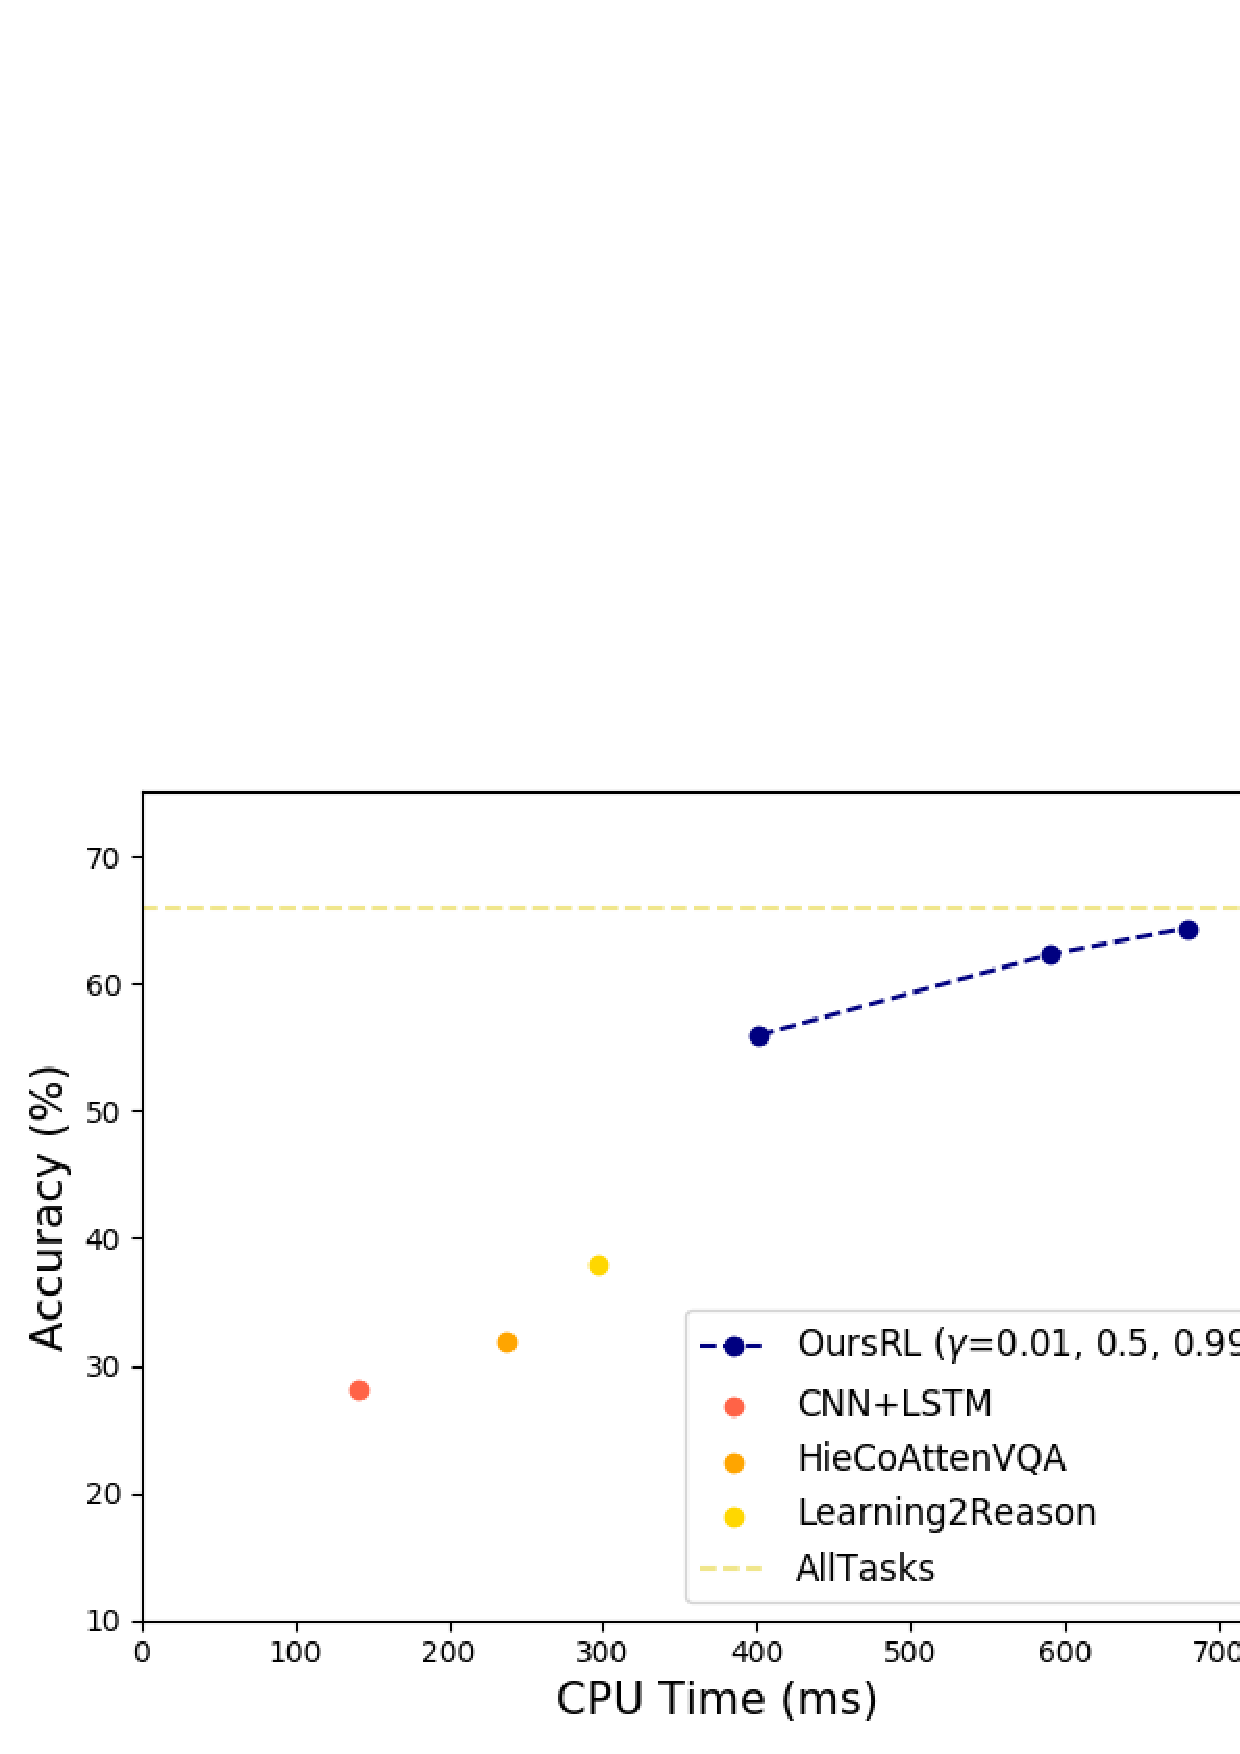
\includegraphics[width=0.9\linewidth]{TimevsAcc.png}
\end{center}
\caption{Inference time and accuracy.}
\label{fig:TimevsAcc}
\end{figure}

%Here to test the generalization, we enlarge the training set by more various question with same meaning. For instance, the original question of $Q_{nl5}$ is \textit{"Who is the defending team?"}, we add three more similar question asking \textit{Who is attacking team?}, \textit{"What is the uniform color of the defending team?"} and \textit{"What is the uniform color of the attacking team?"}. Unlike state-of-art methods answering questions in~\cite{peixi2019}, adding generalization and variation in question would not dramatically change the performance, it is because the structure is not fixed, all the visual task selection is question oriented. For~\cite{hu2017learning}, even though the network is not fixed, the answering part is based on neural network, and essentially it also learns the statically correlation, which leads to the weakness in logical reasoning.

\subsection{Effectiveness of Inference} 
\begin{figure}[tb!]
\centering
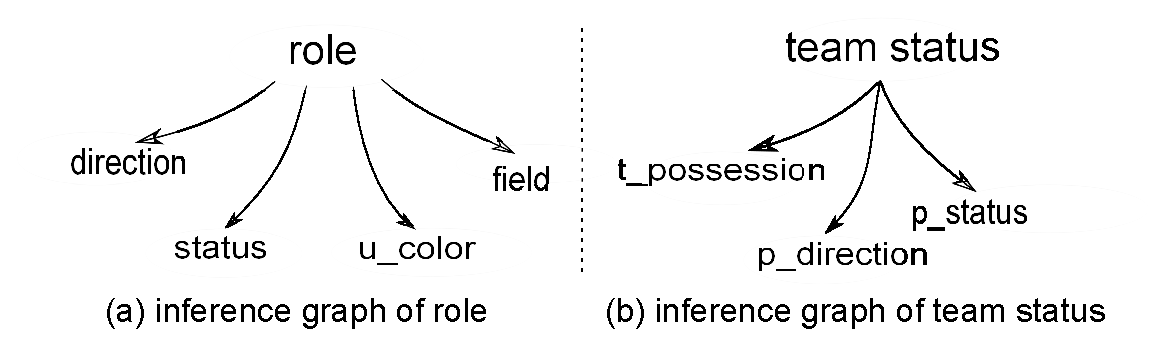
\includegraphics[width=\columnwidth]{PredictNB.eps}
\vspace{-2ex}
\caption{Inference graphs}
\vspace{-2ex}
\label{fig:inferGraph}
\end{figure}


In VQA task, we aim to achieve great performance with short responding time. “CPU Time” evaluates the time cost from features extraction to question answering. All the computation work is implemented on CPU.

In terms of system accuracy, we follow the F-measure. Define that $\#true\_value\_inferred$ is the total number of instances whose attribute $A$ is ``$v$'' and is inferred correctly as ``$v$'', $\#true\_value\_instance$ is the number of all the instances with attribute $A$ of value ``$v$'', and $\#inferred\_instances$ indicates the total number of instances whose attribute $A$ is inferred as ``$v$''. The inference accuracy can be defined as below. 
\begin{equation}
\scriptsize
\color{red}
Acc(A=``v") = \frac{2 \cdot (recall(A=``v")) \cdot presision (A = ``v")}{recall(A=``v") + presision (A = ``v")}
\end{equation}
where:
\begin{equation*}
\begin{split}
recall(A=``v") & = \frac{\#true\_value\_inferred}{\#true\_value\_instance} \\
precision(A=``v") & = 
\frac{\#true\_value\_inferred}{\#inferred\_instance}
\end{split}
\end{equation*}

We compare our approach to the state-of-the-art systems, i.e. CNN+LSTM[???], HieCoAttenVQA[???], and Learning2Reason[???]. 

%==========Table===================
\begin{table}[htbp]
	\renewcommand{\arraystretch}{1}
	\begin{center}
		\small		
		\begin{tabular}{c|*{2}{c}}
			\Xhline{1pt}
			  & Time (ms)  & Acc (\%) \\ \Xhline{0.7pt}
			CNN+LSTM  &  141  &  28.14\\
			HieCoAttenVQA  &  237  &  31.92\\
			Learning2Reason  &  297  &  38.00\\
			Ours (without RL)  &  N/A  &  65.85\\
			Ours ($\gamma=0.01$)  &  401  &  55.92\\
			Ours ($\gamma=0.50$)  &  591  &  62.29\\
			Ours ($\gamma=0.99$)  &  680  &  64.02\\
			\Xhline{1pt}
		\end{tabular}
	\caption{Inference time and accuracy comparison.}
	\label{tab:AccuracyCmp}
	\end{center}
\end{table}
%==========Table===================

\autoref{tab:AccuracyCmp} lists the time cost and accuracy results among different approaches. For CNN+LSTM, HieCoAttenVQA, and Learning2Reason, their systems work quite efficient with responding time less than 300ms. But the accuracies of these three approaches are lower than 40\%, which is unacceptable. Whereas, the system similar to \cite{peixi2019} outperforms all other methods and reaches 65.86\% accuracy, but it costs much more time. Our approach is able to keep balance between effectiveness and efficiency. For effectiveness, our approach achieves 64.02\% accuracy, which is 35.88\%, 32.10\% and 26.02\% higher than results of CNN+LSTM, HieCoAttenVQA, and Learning2Reason, respectively. For efficiency, our approach can reduce the inference time by choosing a small value of $\gamma$.


\stitle{Accuracy of Role}

Based on questions and image characteristics, four variables including $direction$, $status$, $field$, and $unique\_color$ (abbr. $u\_color$) are adopted to calculate conditional probabilities. The inference graph is shown in \autoref{fig:inferGraph} and the inference results are given in \autoref{tab:InferAccRole}. It is easy to find that the inference accuracy for role player reaches 99\%, which is highest among all roles. And the accuracies for different roles are all above 85\%.

%. Note that the domain of variables $direction$, $status$ and $field$ are given in {\color{red}Table ????}, while variable $u\_color$ can have one of two values, to indicate whether a person object has the unique uniform color (=``$U$'') or not (=``$M$'').

%==========Table===================
\begin{table}[htbp]
	\renewcommand{\arraystretch}{1}
	\begin{center}
		\small		
		\begin{tabular}{c|*{3}{r}}
			\Xhline{1pt}
			Role & Precision  & Recall  & Acc \\ \Xhline{0.7pt}
			Goalkeeper  &  94.4  &  85.5  &  89.8\\
			Referee  &  87.4  &  82.8  &  85.0\\
			Player  &  98.8  &  99.3  &  99.0\\
			\Xhline{1pt}
		\end{tabular}
	\caption{Inference accuracy of role (\%).}
	\label{tab:InferAccRole}
	\end{center}
\end{table}
%==========Table===================

Using the conditional probabilities, $VI$ {\color{red}(???)} infers role of each person object. The inference accuracy is shown in \autoref{tab:InferAccRole}. It is easy to find that the inference accuracy for role player reaches 99\%, which is highest among all roles. And the accuracies for different roles are all above 85\%.

\stitle{Accuracy of Team Status}

%===================== figure ============
\begin{figure}[!bth]
	%\scriptsize
	\centering	
	\begin{minipage}[b]{\linewidth}
		\centerline{\includegraphics[width=0.5\linewidth]{example-image-a}}
	\end{minipage}\hfill
	\caption{Attributes of team inference graph.}
	\label{fig:AtribTeamGraph}
\end{figure}
%===================== figure ============

%==========Table===================
\begin{table}[htbp]
	\renewcommand{\arraystretch}{1}
	\begin{center}
		\small		
		\begin{tabular}{c|*{3}{r}}
			\Xhline{1pt}
			 Team Status & Precision  & Recall  & Acc \\ \Xhline{0.7pt}
			Defending  & 89.8 &	74.2 &	81.3\\
			Attacking  &  79.1 & 	92.1 &	85.1\\
			\Xhline{1pt}
		\end{tabular}
		\caption{Inference accuracy of team status (\%).}
		\label{tab:InferAccTeam}
	\end{center}
\end{table}
%==========Table===================

\autoref{tab:InferAccTeam} gives the performance of our approach for inferring team status. 
%Both of the accuracies of defending and attacking are above 80\%. 
In general, inference results of defending and attacking are both above 80\% accuracy.
To be specific, the accuracy for inferring if a team is attacking achieves 85.1\%, which is higher than the inference accuracy for defending status detection by 3.8\%.


\stitle{Accuracy of Field Scene}

%===================== figure ============
\begin{figure}[!bth]
	%\scriptsize
	\centering	
	\begin{minipage}[b]{\linewidth}
		\centerline{\includegraphics[width=0.5\linewidth]{example-image-a}}
	\end{minipage}\hfill
	\caption{Attributes of scene inference graph.}
	\label{fig:AtribSceneGraph}
\end{figure}
%===================== figure ============

Field Scene includes four different scenes, \textit{i.e.} corner kick, free kick, penalty kick and kick-off. Practically, corner kick scene always happens as a single player kick the ball within a one-yard radius of the corner flag and most of players gather in the penalty field. Free kick happens outside the penalty area and defensive wall exists mostly. It is much typical for the penalty kick scene because most of players are out of penalty area except kick player and goalkeeper with football in the penalty spot. As for kick-off scene, the ball is played in the center spot with all members of the opposing team at least 10 yards from the ball. Based on these observations, we design an inference graph in \autoref{fig:AtribSceneGraph}.


Inference results are indicated in \autoref{tab:InferAccField} based on inference graph in \autoref{fig:AtribSceneGraph}. As is shown, the inference accuracy of corner kick, free kick, kick-off and penalty kick are 59.57\%, 63.16\%, 85.94\% and 60.00\%, respectively. It is obvious that the scene of kick off reaches the highest accuracy among all.
 

%==========Table===================
\begin{table}[htbp]
	\renewcommand{\arraystretch}{1}
	\begin{center}
		\small		
		\begin{tabular}{c|*{3}{r}}
			\Xhline{1pt}
			Field Type & Precision  & Recall  & Acc \\ \Xhline{0.7pt}
			Corner-kick &  59.57  &  68.29  &  63.64\\
			Free-kick  &  63.16  &  58.54  &  60.76\\
			Kick-off &  85.94  &  82.09  &  83.97\\
			Penalty-kick  &  60.00  &  60.00  &  60.00\\
			\Xhline{0.7pt}
			Ave.  &  71.28  &  70.73  &  70.89\\
			\Xhline{1pt}
		\end{tabular}
	\caption{Inference accuracy of field scene with the proposed approach (\%).
		% Here ``Co'', ``Fr'', ``Ki'' and ``Pe'' indicate corner kick, free kick, penalty kick and kick-off, respectively.
	}
	\label{tab:InferAccField}
	\end{center}
\end{table}
%==========Table===================


In addition, we compare our approach with NuSVC, MLP, and AdaBoost in \autoref{tab:AccFieldCmp}. The results show that the average accuracy of our approach is higher than that of NuSVC and AdaBoost by 4.49\% and 5.97\% respectively, and slightly better than that of MLP.

%==========Table===================
\begin{table}[htbp]
	\renewcommand{\arraystretch}{1}
	\begin{center}
		\small		
		\begin{tabular}{c|*{3}{r}}
			\Xhline{1pt}
			 & Precision  & Recall  & Acc \\ \Xhline{0.7pt}
			NuSVC  &  68.30  &  65.85  &  66.40\\
			MLP  &  70.80  &  \textbf{70.73}  &  70.32\\
			AdaBoost  &  65.50  &  65.24  &  64.92\\ %\Xhline{0.7pt}
			Ours  &  \textbf{71.28}  &  \textbf{70.73}  &  \textbf{70.89}\\
			\Xhline{1pt}
		\end{tabular}
	\caption{Average accuracy comparison of field scene (\%).}
	\label{tab:AccFieldCmp}
	\end{center}
\end{table}
%==========Table===================



%\stitle{Accuracy of Kick-Off}. {\color{red} SHOW INFERENCE GRAPH AND RESULT TABLE!}
%
%\stitle{Accuracy of Penalty Kick}. {\color{red} SHOW INFERENCE GRAPH AND RESULT TABLE!}
%
%\stitle{Accuracy of Corner Kick}. {\color{red} SHOW INFERENCE GRAPH AND RESULT TABLE!}
%
%\stitle{Accuracy of Attacking Free Kick}. {\color{red} SHOW INFERENCE GRAPH AND RESULT TABLE!}
%
%\stitle{Accuracy of Balls}. {\color{red} Over new dataset. SHOW INFERENCE GRAPH AND RESULT TABLE!}

\subsection{Overall Performance}
\label{sec-overall-performance}
%We use the same question setting as~\cite{peixi2019}, compared the following state-of-the-art methods: \cite{VQA},and~\cite{hu2017learning} with our method ($\gamma$=0.99), the overall performance is shown in Table~\ref{table:stateofart}. 

We compare our proposed method with the following state-of-art methods: LSTM+CNN, HieCoAttenVQA, and Learn2Reason. The results are listed in \autoref{table:stateofartSoc}. The average accuracy using our approach is higher than that of CNN+LSTM, HieCoAttenVQA and Learn2Reason by 20.35\%, 17.64\% and 15.67\%,  respectively. 

%==========Table===================
\begin{table}[htbp]
	\renewcommand{\arraystretch}{1}
	\begin{center}
		\small		
		\begin{tabular}{c|*{4}{c}}
			\Xhline{1pt}
			& CNN+LSTM & HieCoAtten & Learn2Reason & Ours \\ \Xhline{0.7pt}
			$Q_{nl1}$ & 44.23    & 43.62         & 31.12        & \textbf{64.86} \\ 
			$Q_{nl2}$ & 71.31    & \textbf{77.66}         & 9.4          & 63.74 \\ 
			$Q_{nl3}$ & 74.58    & \textbf{83.78}         & 83.21        & 70.00 \\ 
			$Q_{nl4}$ & 40.48    & 39.29         & 51.92        & \textbf{62.14} \\ 
			$Q_{nl5}$ & 49.19    & 49.90         & 30.78        & \textbf{62.58} \\ 
			$Q_{nl6}$ & 20.56    & 18.70         & 30.0         & \textbf{93.33} \\ 
			$Q_{nl7}$ & 11.08    & 12.63         & 36.69        & \textbf{50.60} \\\Xhline{0.7pt} 
			Avg.       & 46.40    & 49.11         & 51.08        & \textbf{66.75} \\
			\Xhline{1pt}
		\end{tabular}
	\caption{Accuracy comparison per question and average for Soccer Dataset (\%).}
	\label{table:stateofartSoc}
	\end{center}
\end{table}
%==========Table===================


%==========Table===================
\begin{table}[htbp]
	\renewcommand{\arraystretch}{1}
	\begin{center}
		\small		
		\begin{tabular}{c|*{4}{c}}
			\Xhline{1pt}
			& CNN+LSTM & HieCoAtten & Learn2Reason & Ours \\ \Xhline{0.7pt}
			$Q_{t1}$  &  63.72  &  64.83  &  \textbf{67.12}  &  65.59\\
			$Q_{t2}$  &  22.87  &  24.52  &  25.04  &  \textbf{82.87}\\
			$Q_{t3}$  &  36.96  &  37.89  &  \textbf{40.12}  &  34.16\\ \Xhline{0.7pt} 
			Avg.       &  50.48  &  51.67  &  53.71  &  \textbf{63.41}\\
			\Xhline{1pt}
		\end{tabular}
		\caption{Accuracy comparison per question type and average for Visual Genome Dataset (\%).}
		\label{table:stateofartVisGen}
	\end{center}
\end{table}
%==========Table===================

To evaluate the generalization of the proposed scheme, we measure its accuracy on Visual Genome Dataset. Results in \autoref{table:stateofartVisGen} show that our approach can handle different types of questions, and the overall performance of our approach surpasses CNN+LSTM, HieCoAttenVQA and Learn2Reason by 12.93\%, 11.74\% and 9.7\%, respectively.
